\sect{Конструкторская часть}
\label{cha:design}

В данном разделе приведены схемы алгоритмов решения задачи коммивояжера: полным перебором и на основе муравьиного алгоритма. 
Также приведена оценка трудоёмкости рассмотренных алгоритмов.

%=====================================================================
\subsect{Разработка алгоритмов}

%На рисунке~\ref{fig:full-comb} представлена схема алгоритма полного перебора.

%\renewcommand{\thefigure}{\thesubsection.\arabic{figure}}
%\begin{figure}[h]
%	\centering
%	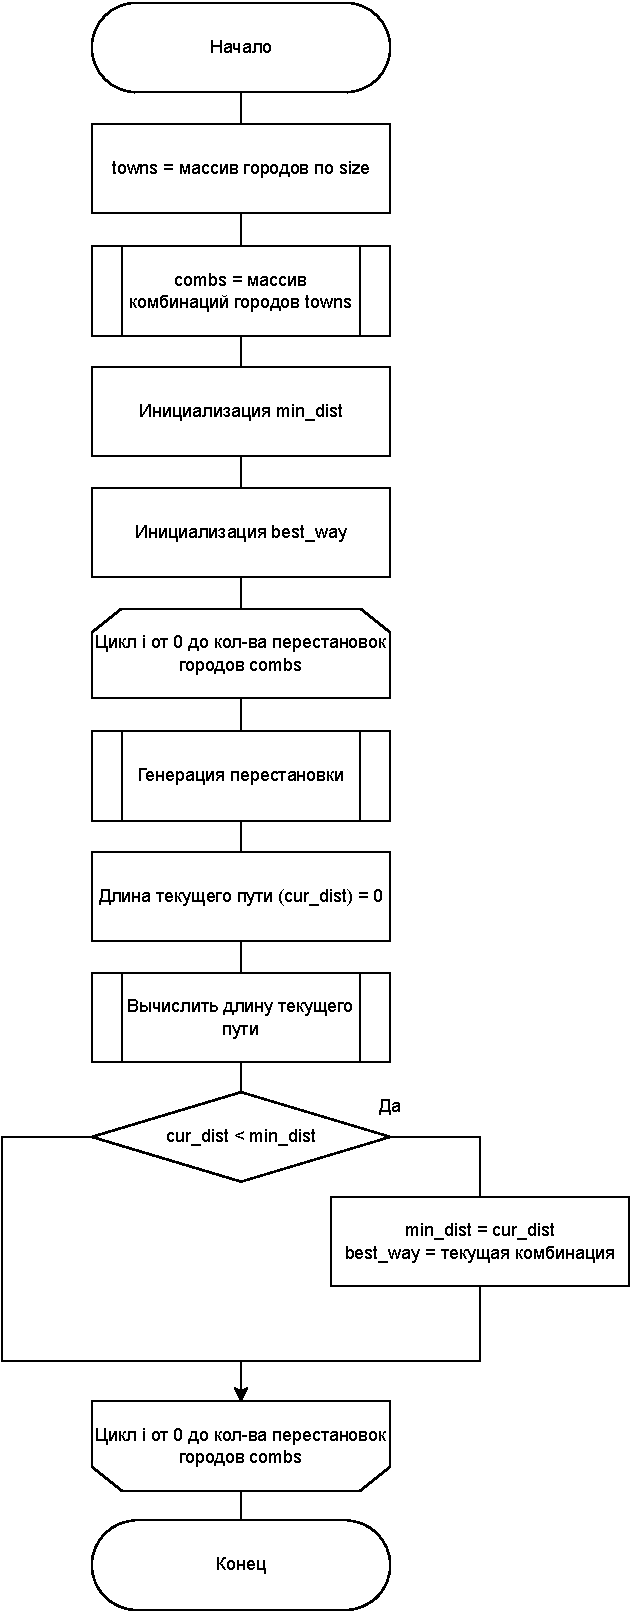
\includegraphics[height=0.9\textheight]{svg/all_combs}
%	\caption{Схема алгоритма полного перебора}
%	\label{fig:full-comb}
%\end{figure}
